\documentclass[final,hyperref={pdfpagelabels=false}]{beamer}
\usepackage{grffile}
\mode<presentation>{\usetheme{I6pd2}}
\usepackage[english]{babel}
\usepackage[utf8]{inputenc}
\usepackage{polski}
\usepackage{amsmath,amsthm, amssymb, latexsym}
\usepackage{graphicx}
\usepackage{epstopdf}
\usepackage{wrapfig}
%\usepackage{times}\usefonttheme{professionalfonts}  % obsolete
%\usefonttheme[onlymath]{serif}
\boldmath
\usepackage[orientation=portrait,size=a0,scale=1.4,debug]{beamerposter}
% change list indention level
% \setdefaultleftmargin{3em}{}{}{}{}{}


%\usepackage{snapshot} % will write a .dep file with all dependencies, allows for easy bundling

\usepackage{array,booktabs,tabularx}
\newcolumntype{Z}{>{\centering\arraybackslash}X} % centered tabularx columns
\newcommand{\pphantom}{\textcolor{ta3aluminium}} % phantom introduces a vertical space in p formatted table columns??!!

\listfiles

%%%%%%%%%%%%%%%%%%%%%%%%%%%%%%%%%%%%%%%%%%%%%%%%%%%%%%%%%%%%%%%%%%%%%%%%%%%%%%%%%%%%%%
\graphicspath{{figures/}}
 
\title{\huge PAAL: Practical Approximation Algorithm Library}
\author{Piotr Jaszkowski, Mateusz Machalica, Grzegorz Prusak and Łukasz Solak}
\institute[University of Warsaw]{The Faculty of Mathematics, Informatics and Mechanics, University of Warsaw, Warsaw, Poland}
\date[May 24, 2013]{May 24, 2013}

%%%%%%%%%%%%%%%%%%%%%%%%%%%%%%%%%%%%%%%%%%%%%%%%%%%%%%%%%%%%%%%%%%%%%%%%%%%%%%%%%%%%%%
\newlength{\columnheight}
\setlength{\columnheight}{105cm}


%%%%%%%%%%%%%%%%%%%%%%%%%%%%%%%%%%%%%%%%%%%%%%%%%%%%%%%%%%%%%%%%%%%%%%%%%%%%%%%%%%%%%%
\begin{document}
\begin{frame}

	\begin{columns}
		\begin{column}{.96\textwidth}
			\vspace{1cm}
			\begin{center}
			\veryHuge Aproksymacje VS Metaheurystyki
			\end{center}
			\vspace{1cm}
		\end{column}
	\end{columns}

	\begin{columns}
		\begin{column}{.46\textwidth}
			\begin{block}{Algorytmy aproksymacyjne}
        Algorytmy służące do znajdowania przybliżonych rozwiązań problemów optymalizacyjnych. Stosuje się je zwykle do rozwiązywania problemów, dla których nie
        są znane szybkie algorytmy znajdujące rozwiązanie dokładne, na przykład dla problemów NP-zupełnych.  Istotą algorytmu aproksymacyjnego, tym co odróżnia
        go od algorytmu heurystycznego, jest gwarantowany poziom przybliżenia rozwiązania optymalnego, zwykle zadany przez pewien stały czynnik.  \vspace{5cm}
			\end{block}
		\end{column}

		\begin{column}{.46\textwidth}
      \begin{block}{Metaheurystyka}
        Ogólny algorytm (heurystyka) do rozwiązywania problemów obliczeniowych, naczęściej optymalizacyjnych -- definiujących pewną funkcję celu nad
        przestrzenią rozwiązań. Poza tą funkcją, metaheurystyki nie korzystają bezpośrednio ze szczególnych własności problemu, stąd łatwo je stosować do
        szerokiej ich gamy. Do metaheurystyk zaliczamy m.in.:
				\begin{itemize}
        \item algorytmy typu Local Search - algorytmy ,,spacerujące'' po przestrzeni rozwiązań zgodnie z pewną topologią w poszukiwaniu lepszych rozwiązań
        \item algorytmy typu Monte Carlo Tree Search - uogólnione algorytmy zachłanne, które do oceny decyzji częściowej używają losowych zejść w dół drzewa
          decyzyjnego.
				\end{itemize}
			\end{block}
		\end{column}
	\end{columns}
	
  \begin{columns}
    \begin{column}{.96\textwidth}
      \vspace{1cm}
      \begin{center}
        \veryHuge starcie nastąpi na następujących problemach
      \end{center}
      \vspace{1cm}
    \end{column}
  \end{columns}

  \begin{columns}
    \begin{column}{.46\textwidth}
      \begin{block}{Metrical Traveling Salesman Problem}
        \begin{minipage}{\linewidth}
          \begin{columns}
            \begin{column}{.38\linewidth}
              Dla danego grafu pełnego i nieujemnej funkcji kosztu określonej na jego krawędziach, spełniającej nierówność trójkąta, należy znaleźć najtańszy
              cykl przechodzący przez każdy z wierzchołków dokładnie raz.
            \end{column}

            \begin{column}{.58\linewidth}
              \begin{figure}
                \centering
                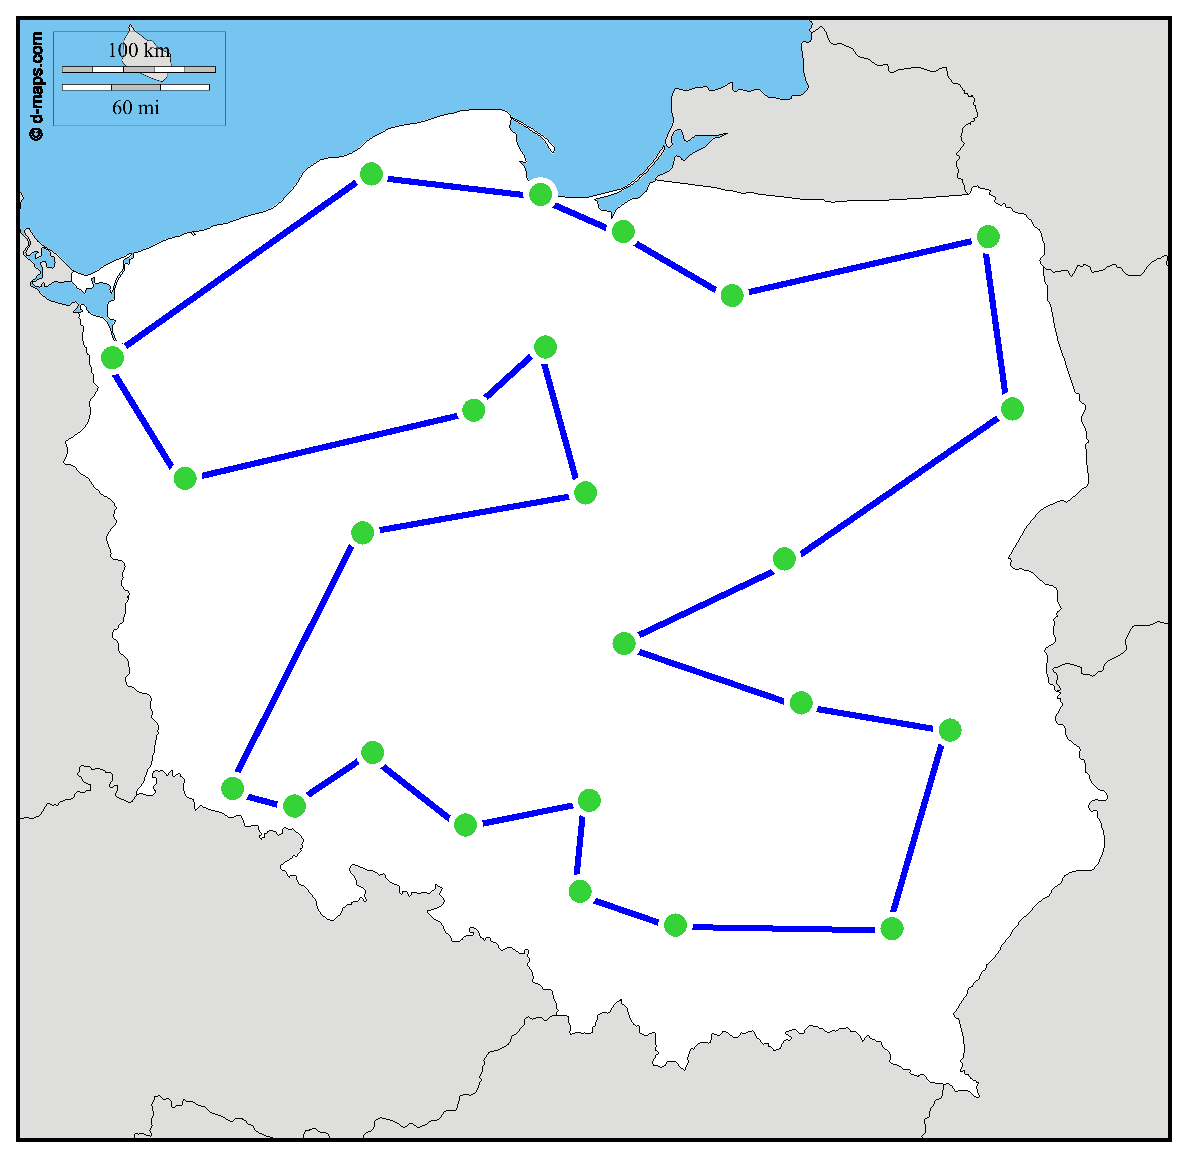
\includegraphics[width=0.8\linewidth]{poland_cities_cycle.eps}
              \end{figure}
            \end{column}

          \end{columns}
        \end{minipage}
      \end{block}

      \begin{block}{Steiner Forest}
        \begin{minipage}{\linewidth}
          \begin{columns}
            \begin{column}{.58\linewidth}
              Dany jest graf nieskierowany $G = (V, E)$, funkcja kosztu $c: E \rightarrow Q^+$ oraz rodzina $S_1, \hdots, S_k$ podzbiorów rozłącznych $V$.
              Należy znaleźć podgraf $G$ o najmniejszym koszcie, w którym wierzchołki należące do tego samego zbioru są połączone.
            \end{column}

            \begin{column}{.38\linewidth}
              \begin{figure}
                \centering
                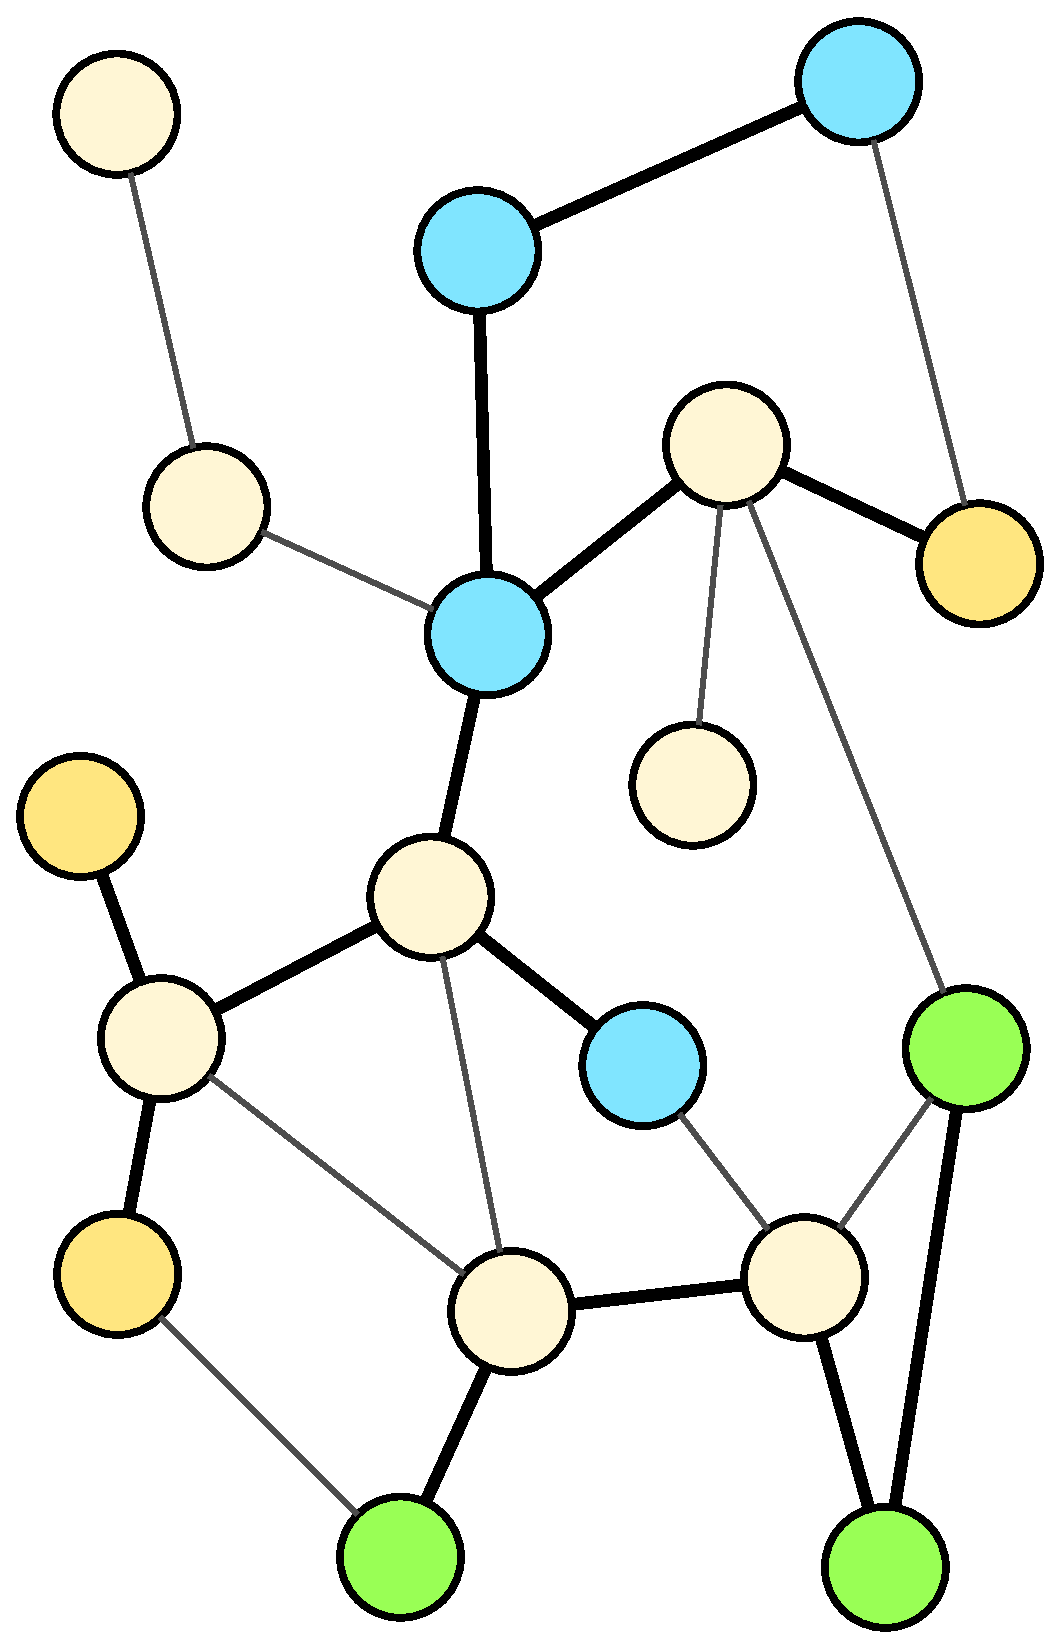
\includegraphics[height=.96\linewidth]{sf_poster.eps}
              \end{figure}
            \end{column}

          \end{columns}
        \end{minipage}
      \end{block}

    \end{column}

    \begin{column}{.46\textwidth}
      \begin{block}{Metrical Uncapacitated Facility Location}
        \begin{minipage}{\linewidth}
          \begin{columns}
            \begin{column}{.58\linewidth} % TODO adjust after insering proper picture
              Niech $G$ będzie grafem dwudzielnym o zbiorze wierzchołków $F \cup C$, gdzie $F$ jest zbiorem obiektów, a $C$ zbiorem miast. Niech $f_i$ będzie kosztem
              otwarcia obiektu $i$, a $c_{ij}$ kosztem połaczenia miasta $j$ z (otwartym) obiektem $i$. Koszty połączeń spełniają nierówność trójkąta. Należy znaleźć
              podzbiór $I \subseteq F$ obiektów, które zostaną otwarte, oraz funkcję $\phi : C \rightarrow I$, która każdemu miastu będzie przypisywała obiekt
              otwarty. Łączny koszt otwarcia obiektów i połączenia miast z obiektami powinien być jak najmniejszy.
            \end{column}

            \begin{column}{.38\linewidth} % TODO adjust after insering proper picture
              \begin{figure}
                \centering
                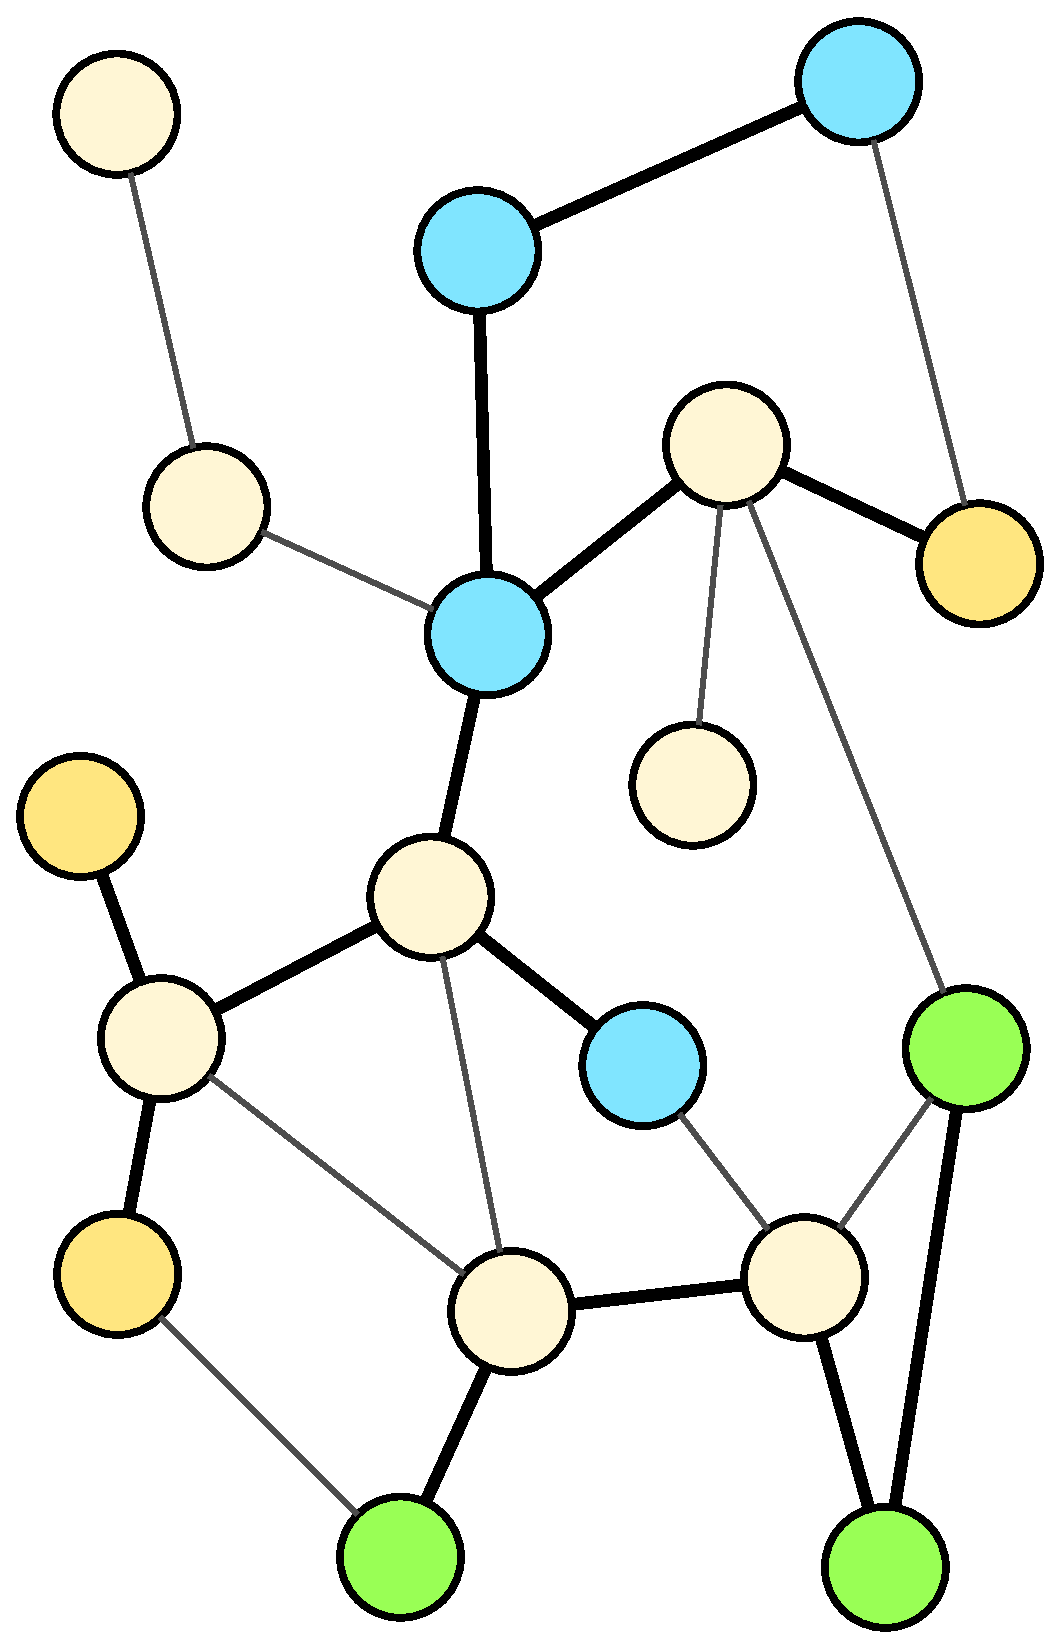
\includegraphics[height=.96\linewidth]{sf_poster.eps} % TODO FL picture
              \end{figure}
            \end{column}

          \end{columns}
        \end{minipage}
      \end{block}
    \end{column}
	\end{columns}
  \vskip1ex
  %\tiny\hfill\textcolor{ta2gray}{Created with \LaTeX \texttt{beamerposter}  \url{http://www-i6.informatik.rwth-aachen.de/~dreuw/latexbeamerposter.php}}
  \tiny\hfill{Created with \LaTeX \texttt{beamerposter}  \url{http://www-i6.informatik.rwth-aachen.de/~dreuw/latexbeamerposter.php} \hskip1em}
\end{frame}
\end{document}


%%%%%%%%%%%%%%%%%%%%%%%%%%%%%%%%%%%%%%%%%%%%%%%%%%%%%%%%%%%%%%%%%%%%%%%%%%%%%%%%%%%%%%%%%%%%%%%%%%%%
%%% Local Variables: 
%%% mode: latex
%%% TeX-PDF-mode: t
%%% End:
% vim: et:sw=2:ts=2:tw=160
